%%%% --------------------------------------------------------------------------
%%
%%          K I L O N O V A
%%
%%%% --------------------------------------------------------------------------
\chapter{Kilonova} \label{ch:kilonova} 

In this chapter we discuss models of the quasi-thermal counterpart 
of the \ac{BNS} mergers, powered by the decay of the newly sythesized heavy 
elements via \rproc{} \nuc{} discussed in the previous chapter \ref{ch:nucleo}.
%
In Sec.~\ref{sec:intro:kilonova} we recalled the origin of the quasi-thermal emission, 
the energy release in nuclear heating, its thermalization in ejecta, and the 
opacities of the latter and how they shape the final emission giving a unique 
signature. 
%

We compute the \ac{kN} light curves via 
semi-analytic, multi-component, asnisotropic code \mkn{} 
\citep{Perego:2017wtu,Barbieri:2019sjc,Breschi:2021wzr},
from the brief description of which we begin the chapter.
%
Then we apply the code \mkn{} to the ejecta from our \ac{NR} \ac{BNS} 
merger simulations and investigate how the newly found ejecta component, the 
\ac{SWW} (see Ch.~\ref{ch:bns_sims}) affects the synthetic light curves and 
compare the result with observations, the \AT{}.

%% =====================================================================================
%%
%%               I N T R O D U C T I O N
%%
%% =====================================================================================

\section{Semi-analytic \ac{kN} model}

We consider the ejecta geometry directly imported from the 
\ac{NR} simulations in a form of the angular profiles 
(assuming axisymmetry).
%with 
%respect to the polar angle and averaging over the azimuthal angle.
In a several cases we also use the analytical ejecta profiles, with 
either smooth of step-like dependency on the polar angle.
%
The viewing angle, $\theta_{\text{obs}}$, is measured as the angle between the 
polar axis and the line of sight of the observer.
%-
% Ejecta profile
Each ejecta component (\eg, \ac{DE}, \ac{SWW}) is described through 
the angular distribution of its ejected mass, $M_{\text{ej}}(\theta)$, 
velocity $\upsilon_{\text{ej}}(\theta)$,
and opacity, $\kappa_{\text{ej}}(\theta)$.
%
The polar angle, $\theta$, measured from the rotational axis, is discretized in 
$N_\theta=30$ angular bins evenly spaced in $\cos{(\theta)}$.
%
Additionally, within each ray, the matter 
has a fixed velocity distribution, 
$\xi(\upsilon) \propto (1 - (\upsilon / \upsilon_{\text{max}})^2)^3$,
%
%\begin{equation}
%\xi(\upsilon) \propto \Big(1 - \left(\frac{\upsilon}{\upsilon_{\text{max}}}\right)^{2}\Big)^{3}, 
%\end{equation}
%
where $\xi(\upsilon) \dd \upsilon$ is the matter contained in an infinitesimal layer of speed 
$\left[\upsilon,\upsilon+\dd \upsilon\right]$, and 
$\upsilon_{\text{max}}=\upsilon_{\text{max}}(\upsilon_{\text{RMS}})$ 
is the maximum velocity at the outermost edge of the component.
%
The characteristic quantities 
%$\varrho$, $\upsilon$ and $\kappa$ 
are then evaluated 
for every bin according to the assumed input profiles.
Then the emitted luminocity is evaluated for every bin 
using the radial model described in \citet{Perego:2017wtu}, and in 
\S{4} of \citet{Barbieri:2019kli}.
%
The model assumes that the thermal radiation is emitted at the photosphere, located at 
$R_{\text{ph}}$, with effective emission temperature $T_{\text{eff}}$ via the 
Stefan-Boltzmann law, \ie, the black-body radiation. This assumption is justified 
when modeling early emission, when the ejecta is hot and opaque. However, at later 
times, as ejecta falls out of \ac{LTE} with its radiation, the assumption breaks.
%

%%%% -----------------------
% Heating rates
%%%% -----------------------
%The time-dependent nuclear heating are approximated as Eq.~\eqref{eq:kilonova:eps_korob}.
%rate $\epsilon_{\text{nuc}}$ \red{assert notations} entering these calculations is approximated 
%by an analytic fitting formula, derived from detailed nucleosynthesis 
%calculations~\citep{Korobkin:2012uy} Eq.~\eqref{eq:kilonova:heat_korob}, 
%modified as follows
%                                            << moved above >>>
%\begin{equation}
%\label{eq:epsnuc}
%\epsilon_{\text{nuc}}(t)= \epsilon_0 \, \frac{\epsilon_{\text{th}}(t)}{0.5} \, \epsilon_{\text{nr}}(t) \,
%\left[ \frac{1}{2} - \frac{1}{\pi} \arctan\left(\frac{t-t_0}{\sigma}\right)\right]^{\alpha}\,,
%\end{equation}
%%
%where $\sigma = 0.11$~s, $t_0 = 1.3$~s, $\alpha=1.3$ and $\epsilon_{\text{th}}(t)$ is the 
%thermalization efficiency tabulated according to \citet{Barnes:2016umi}.
%\red{$\epsilon_0$ is not introduced. Is it a constant?}
%%
%The heating factor $\epsilon_{\text{nr}}(t) $ is introduced as in \citet{Perego:2017wtu} to roughly adjust 
%the Eq.~\eqref{eq:epsnuc} in the regime of mildly neutron-rich matter (characterized by an initial 
%electron fraction $Y_e \gtrsim 0.25$), \citep[see, \eg][]{Martin:2015hxa}:
%%
%\begin{equation}
%\label{eq:epsnr}
%\epsilon_{\text{nr}}(t,\kappa) = \left[1-w(\kappa)\right] + w(\kappa)\,\epsilon_{Y_e}(t)\,,  
%\end{equation}
%%
%where $w(\kappa)$ is a logarithmic smooth clump function such that $w(\kappa < 1~\igscm) = 1$ and 
%$w(\kappa > 10~\igscm)=0$ and the factor $\epsilon_{Y_e}(t)$ accounts for the dependency on $Y_e$:
%if $Y_e < 0.25$, then $\epsilon_{Y_e}(t)=1$, otherwise, when $Y_e \ge 0.25$,
%%
%\begin{equation}
%\label{eq:epsye}
%\epsilon_{Y_e}(t) =\epsilon_{\text{min}}+{\epsilon_{\text{max}}}{\left[1+ e ^{4(t/t_\epsilon-1)}\right]}^{-1}\,,
%\end{equation}
%%
%where $t_\epsilon = 1~{\text{day}}$, $\epsilon_{\text{min}}=0.5$ an $\epsilon_{\text{max}} = 2.5$.


%% FROM Breschi et al (from perego et al)

\begin{figure}
    \centering 
    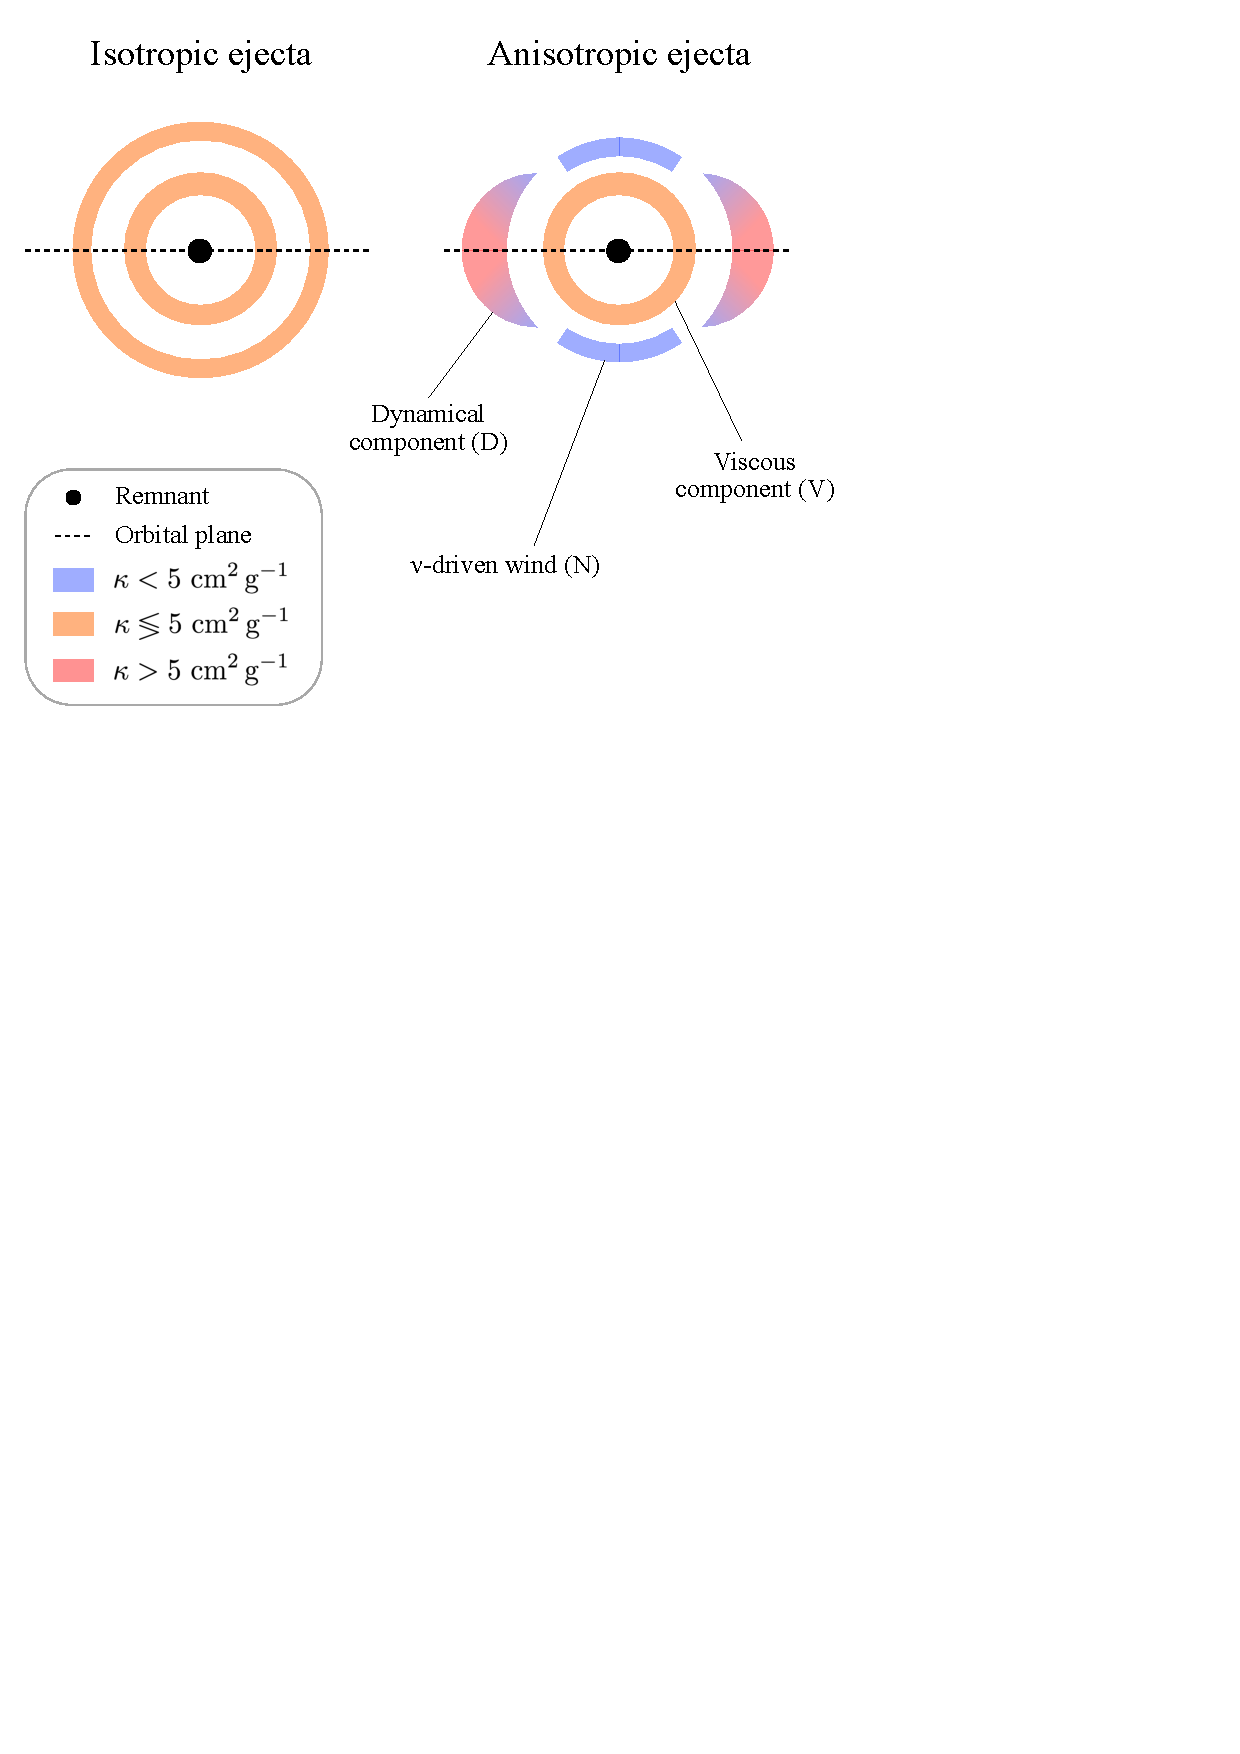
\includegraphics[width=0.58\textwidth]{profiles_op.pdf}
    \caption{Graphic representation of the analyzed
        ejecta profiles for isotropic and anisotropic cases
        from an azimuthal perspective and for a fixed moment of time.
        The black dot represents the remnant and the dashed line is the projected orbital
        plane of the binary. The shadowed areas describe the ejecta profiles: the shape
        characterizes the mass distribution, while the colors refer to 
        the prior assumptions on the opacity parameter.
        In particular, blue regions denote opacities lower than $5~\igscm$,
        red regions refer to opacities greater than $5~\igscm$,
        and oranges areas indicate a broadly distributed opacity.
        All shells are isotropically expanding with a constant velocity.
        (Adapted from \citet{Breschi:2021wzr})
    }
    \label{fig:cartoon}
\end{figure}


For a neutron-rich ejecta, $Y_e\leq 0.2$, the heating rate is dominated by a large statistical 
ensemble of nuclei, however at higher $Y_e\gtrsim 0.2$ corrections are required. 
The time-dependent nuclear heating rate $\epsilon_{\text{nuc}}$ 
%\red{assert notations} 
can be approximated via an analytic fitting formula, derived from detailed nucleosynthesis 
calculations~\citep{Korobkin:2012uy}  
%
\begin{equation}
\label{eq:kilonova:eps_korob}
\epsilon_{\text{nuc}}(t)= \epsilon_0 \, \frac{\epsilon_{\text{th}}(t)}{0.5} \, \epsilon_{\text{nr}}(t) \,
\left[ \frac{1}{2} - \frac{1}{\pi} \arctan\left(\frac{t-t_0}{\sigma}\right)\right]^{\alpha}\,,
\end{equation}
%
where $\sigma = 0.11\,$s, $t_0 = 1.3\,$s, $\alpha=1.3$,
$\epsilon_0$ is the constant and 
$\epsilon_{\text{th}}(t)$ is the 
thermalization efficiency tabulated according to \citet{Barnes:2016umi}.
%
The heating factor $\epsilon_{\text{nr}}(t) $ is introduced as in \citet{Perego:2017wtu} to roughly adjust 
the Eq.~\eqref{eq:kilonova:eps_korob} tp the regime of mildly neutron-rich 
matter (characterized by an initial 
electron fraction $Y_e \gtrsim 0.25$), \citep[see, \eg][]{Martin:2015hxa}, 
%
\begin{equation}
\label{eq:epsnr}
\epsilon_{\text{nr}}(t,\kappa) = \left[1-w(\kappa)\right] + w(\kappa)\,\epsilon_{Y_e}(t)\,,  
\end{equation}
%
where $w(\kappa)$ is a logarithmic smooth clump function such that $w(\kappa < 1~\igscm) = 1$ and 
$w(\kappa > 10~\igscm)=0$ and the factor $\epsilon_{Y_e}(t)$ accounts for the dependency on $Y_e$:
if $Y_e < 0.25$, then $\epsilon_{Y_e}(t)=1$, otherwise, when $Y_e \ge 0.25$,
%
\begin{equation}
\label{eq:epsye}
\epsilon_{Y_e}(t) =\epsilon_{\text{min}}+{\epsilon_{\text{max}}}{\left[1+ e ^{4(t/t_\epsilon-1)}\right]}^{-1}\,,
\end{equation}
%
where $t_\epsilon = 1~{\text{day}}$, $\epsilon_{\text{min}}=0.5$ an $\epsilon_{\text{max}} = 2.5$.

%%%% --------------
% Opacity 
%%%% --------------
%
The mean plank opacities for the hot ejecta are adopted from the systematic study 
(see Figure.~4 in \citet{Tanaka:2019iqp}).
%Notably, the atomic opacity depends on its ionization state. %\red{might reference Barns work}.
When temperature drops and atoms become neutral, the photon opacity sharply decreases. 
This was shown to have a strong effect on 
\acp{LC} in high-frequency bands, \eg, $V$, $U$, $B$ and $g$ \citep{Villar:2017oya}. In order to account 
for the drop in opacity when the temperature falls below the certain value that corresponds to the full 
recombination, the $T_{\text{floor}}$ is introduced \citep{Kasen:2017sxr,Kasen:2018drm} as a minimum value that 
$T_{\text{eff}}$ can have. Due to the presence of lanthanides in the ejcta, 
we consider two floor temperatures, 
depending on the composition: the $T_{\text{floot}}^{\text{Ni}}$ and $T_{\text{floot}}^{\text{La}}$ for 
the lanthanides free and rich ejecta respectively.

%----  EATS integrator
The emission coming from the different angular bins is combined to obtain the spectral flux at the observer location as, 
%
\begin{equation}
\label{eq:spectral_flux}
F_{\nu}(\mathbf{n},t) = \int_{\mathbf{n}_{\Omega} \cdot \mathbf{n}> 0} 
\left( \frac{R_{\text{ph}}(\Omega,t)}{D_L} \right)^2  B_{\nu}(T_{\text{eff}}(\Omega,t))~\mathbf{n} \cdot  \dd\boldsymbol{\Omega}\, , 
\end{equation}
%
where $\mathbf{n}$ is the unitary vector along the line of sight, $\mathbf{n}_{\Omega}$ is the unitary 
vector spanning the solid angle $\Omega$, $D_L$ is the luminosity distance, $R_{\text{ph}}$ is the local 
radial coordinate of the photospheric surface, and $B_{\nu}(T_{\rm eff})$ is the spectral radiance at 
frequency $\nu$ for a surface of temperature $T_{\text{eff}}$. 
%
% ---- Magnitudes
We also make use of the apparent AB magnitude mag$_b$ in a given photometric band $b$, defined as:
%
\begin{equation}
\label{eq:mag}
\text{mag}_b(\mathbf{n},t) = -2.5 \log_{10}\left( F_{\nu_b}(\mathbf{n},t) \right)-48.6\,,
\end{equation}
where $\nu_b$ is the effective central frequency of band $b$.





%% =====================================================================================
%%
%%               R E S U L T S
%%
%% =====================================================================================

%In the following we perform two types of the analysis (i) the fully \ac{NR}-informed \ac{kN} models, where the the only ejecta components considered, are those found in simulations and (ii) the parametric \ac{kN} models, where we use the analytic ejecta profiles, with the parameters obtained from fitting formulae (see Ch.~\ref{ch:stat_anal}).

\begin{figure}[t]
    \centering
    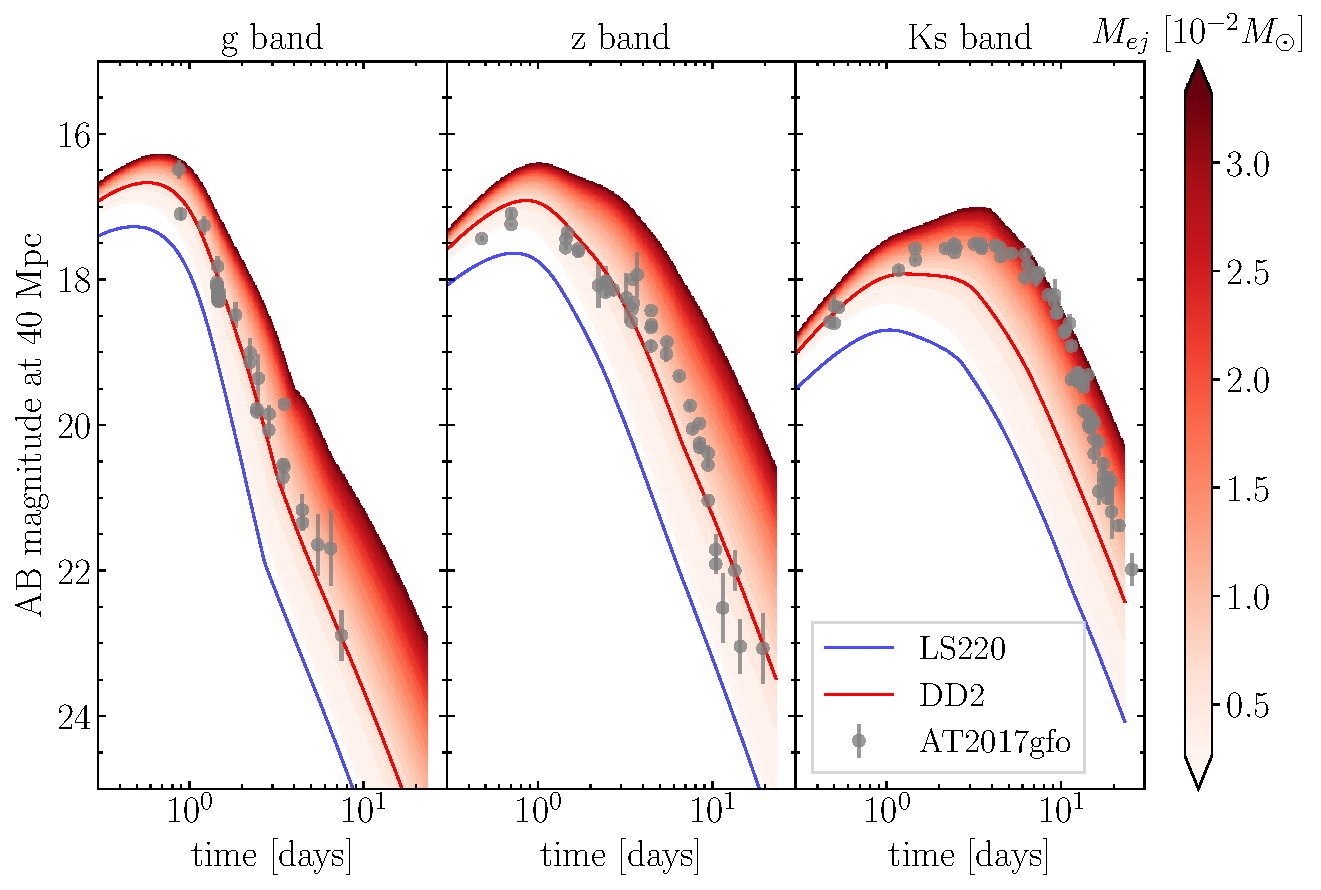
\includegraphics[width=0.75\textwidth]{kilonova/mkn_dd2_band.pdf}
    \caption{Bolometric kN light curves in three representative bands from blue to
        infrared for the two simulations with turbulence viscosity compared to
        \AT{} data from~\citep{Villar:2017wcc}.
        The color gradient is the effect related to different
        \ac{SWW} masses, that suggests possible variations of the light
        curves for different \ac{BNS}. The band is computed by extracting the
        \ac{SWW} mass from DD2 every $10$~ms until the end of the simulation, and
        then by linearly extrapolating the data to $250$~ms.
        (Adapted from \citet{Nedora:2019jhl})
    }
    \label{fig:knlc}
\end{figure}


\section{\ac{SWW} for the blue component of \AT{}}\label{sec:kilonova:result}

The \ac{BNS} merger ejecta consists of several anisotropic components with different 
properties (see the discussion in Sec.~\ref{sec:intro:ejecta} and Chapter~\ref{ch:bns_sims}).
%
%Hence, the \ac{kN} model ought to account for the anisotropy of the ejecta composition. Additionally, the interaction between components needs to be included, but we leave this to future works.
%% ---
Indeed, outflow properties inferred for \AT{} using multi-components and 2D \ac{kN} models including the ejecta anisotropy and cross-component irradiation are broadly compatible with the results from simulations, \eg, \citep{Kawaguchi:2018ptg}, see also Sec.~\ref{sec:intro:kilonova}. 
%% ---
The particular challenge however, is to reproduce the early blue emission. 
Both semi-analytical and radiation transport
models require ejecta properties different from those found in
simulations. In particular, 
this component requires fast low opacity, massive ejecta \citep{Fahlman:2018llv} that is generally 
not found in \ac{BNS} simulations.
%% ---
Notably, the early blue component can be explained by the emission arising 
in the interaction between a relativistic jet and the ejecta
\citep{Lazzati:2016yxl,Bromberg:2017crh,Piro:2017ayh}.
However, simulations show that that successful jets do not deposit a sufficient amount of thermal energy in the ejecta for this mechanism to work \citep{Duffell:2018iig}. 
Other possibilities include the presence of highly magnetized winds \citep{Metzger:2018uni,Fernandez:2018kax},
or the presence of the so-called viscous dynamical ejecta \citep{Radice:2018ghv}.
These two explanations require the development of large-scale strong magnetic fields.
%% ---
In this section we show that the presence of the massive \ac{SWW},
found in the ab-initio \ac{BNS} merger simulations with long-lived \ac{NS} remnants 
(see Chapter~\ref{ch:bns_sims}) can help explain the early blue emission, 
relaxing the need for strong ordered magnetic fields. 


We begin by considering two equal mass \ac{NR} \ac{BNS} merger models with LS220 
and DD2 \acp{EOS}, that produce short and long-lived \ac{NS} remnant respectively. 
Using the \texttt{MKN} code, discussed above, we construct \ac{NR}-informed 
\acp{LC} for both, \ac{DE} only and the combination of \ac{DE} and \ac{SWW}\footnote{
    The \texttt{MKN} code does not include the effects of multiple ejecta component 
    iteration. We leave this to future works.
}.
%%% ---
%For both models we produce \ac{NR}-informed \acp{LC}, using both the \ac{DE} and \ac{SWW} for the model with the long-lived \ac{MNS} remnant, and \ac{DE} only for the model with the short-lived one.
%% ---
The result is shown in Fig.~\ref{fig:knlc}.
We observe, that the \ac{DE} only is insufficient to explain the \AT{} in 
all bands considered irrespective of the \ac{BNS} model. However, the informed 
by both \ac{DE} and \ac{SWW} \ac{LC} of the DD2 $q=1.00$ (\texttt{SR}) model 
is sufficiently bright to account for the emission in 'z' band. 
%% However, it appears dimmer than the early blue \AT{} emission in 'g' band. 
%% ---
The emission in low frequency bands requires a more massive 
\ac{SWW} with mass ${\gtrsim} 2\times10^{-2}M_{\odot}$, implying a remnant lifetime of ${\gtrsim}200$~ms, as the \ac{SWW} mass flux is present as long 
as \ac{MNS} remnant is present (see Sec.\ref{sec:bns_sims:mj_loss}).
However, a more massive \ac{SWW} is incompatible with
the early emission for the low-frequency bands of \AT{}.
%% --- 
In order to explain the late emission in the low frequncy bands and 
early emission in high frequency bands, a combination of the \ac{SWW} and 
viscous ejecta from the disintegration of the disk are required.
%% --- 
Our results, however have uncertainties related to our simplified calculation of
the \ac{kN} \acp{LC} which is expected to be less accurate at
late times when absorption features and deviations from \ac{LTE} become more relevant \citep[see \eg][]{Smartt:2017fuw}.
To model the \ac{kN} emission more robustly, the time- and energy-dependent 
photon radiation transport models are required 
\citep{Kasen:2017sxr,Tanaka:2017qxj,Miller:2019dpt,Bulla:2019muo}.
Additionally, the systematic uncertainties in
nuclear (\eg, mass models, fission fragments and $\beta$-decay
rates) and atomic (\eg, detailed wavelength dependent opacities for
\rproc{} element) physics enter all the current \ac{kN} models 
\citep{Eichler:2014kma,Rosswog:2016dhy,Gaigalas:2019ptx}.




%\subsection{Conclusion}
%
%\red{Copied}
%Standard kN models applied to the early AT2017gfo light curve are in
%tension with ab-initio simulations conducted so far.
%While alternative interpretations have been proposed, they are either
%disfavored by current simulations and observations (e.g. jets) \citep{Bromberg:2017crh,Duffell:2018iig},
%or require the presence of large-scale strong magnetic 
%fields which might not be formed in the postmerger
%\citep{Metzger:2018uni,Fernandez:2018kax,Radice:2018ghv,Ciolfi:2019fie}. 
%We identified a robust dynamical mechanism for mass ejection that
%explains early-time observations without requiring any fine-tuning.
%The resulting nucleosynthesis is complete and produces all
%$r$-process elements in proportions similar to solar system abundances.
%Methodologically, our work underlines the importance of employing
%NR-informed ejecta for the fitting of light-curves.
%Further work in this direction should 
%include better neutrino-radiation transport and magnetohydrodynamic effects
%\citep{Siegel:2017nub,Fujibayashi:2017puw,Radice:2018xqa,Radice:2018pdn,Miller:2019dpt}. 


\section{Fit-informed kilonova models}


%% KILONVA PLOTS
\begin{figure*}[t]
    \centering 
    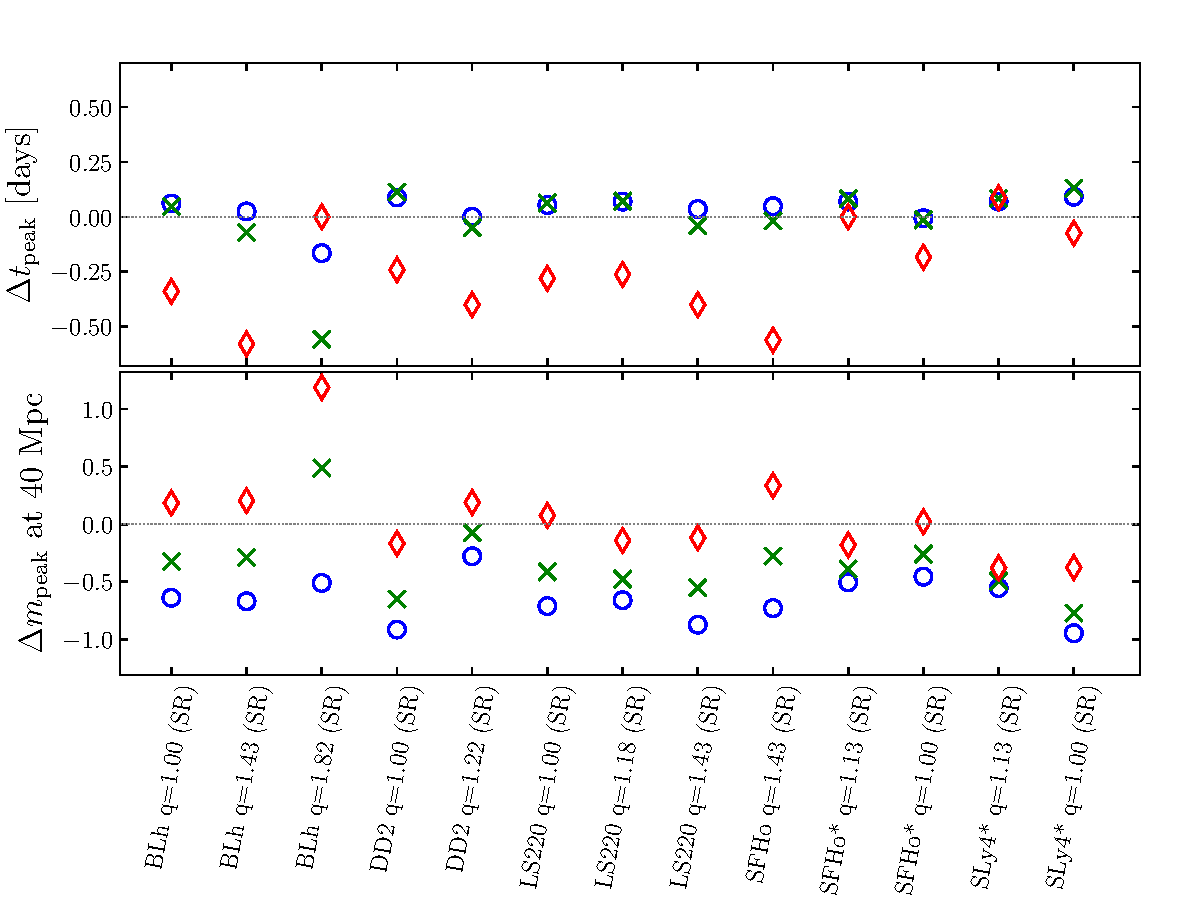
\includegraphics[width=0.49\textwidth]{kilonova/mkn_multiband_dyn_NR.pdf}
    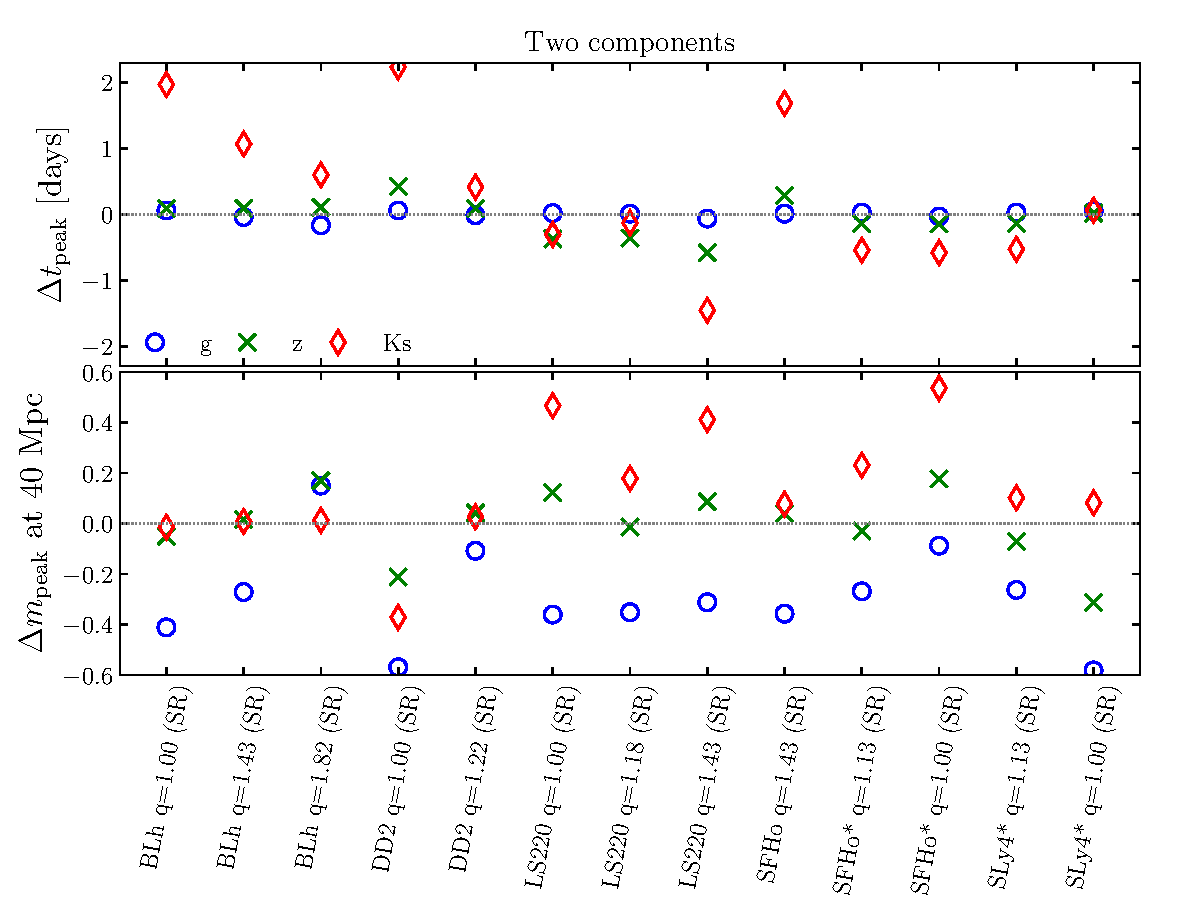
\includegraphics[width=0.49\textwidth]{kilonova/mkn_multiband_dynsec_NR.pdf}
    \caption{
        Comparison between one component light curves (\textit{left panel}) and
        two components light curves (\textit{right panel}) in $g$, $z$ and $K_s$
        bands using direct NR input or the fitting formulae for the
        dynamical ejecta and disk mass. 
        The $y-$axis displays the difference between the peak time 
        (\textit{top panel}), $\Delta t_{\rm peak} = t_{\rm peak; NR} - t_{\rm peak; fit}$, 
        and peak magnitude, $\Delta m_{\rm peak} = m_{\rm peak; NR} - m_{\rm peak; fit}$, 
        (\textit{bottom panel});
        the $x-$axis shows selected BNS models of \DSrefset{}.
        The fits employed here are the polynomials in $(q,\tilde{\Lambda})$ used with the 
        best fitting coefficients, calibrated to \DSheatcool{} (that includes \DSrefset{}).
        The plot shows that 
        the light curves generated with the dynamical ejecta fits (one
        component) tend to underestimate the peak times and magnitudes
        of NR-informed light curves, especially in the $K_s$ band. In case of 
        dynamical ejecta and disk wind (two
        components) light curves, the peak
        time is less constrained ($\pm 2$~days) in the $K_s$ band, but the
        peak magnitudes is predicted more accurately $\pm0.5$~mag. }
    %% \vn{Note! That for NR-informed lightcurves \textbf{full} NR ejecta profile (for dyn. ej.)
    %% is fed into MKN. Thus here the geometric effects and poor fit performance contribute to the
    %% qdeviation.}
    \label{fig:mkn_example}
\end{figure*}

%In this section we investigated statistical properties of the \ac{DE} and remnant from 
%several sets of \ac{NR} \ac{BNS} models. 
%
%The analysis showed that the properties of the ejecta and remnant disk mass are subjected 
%to large systematic uncertainties that stem from difference in input physics: neutrino 
%treatment and \ac{EOS}.
%%
%Additionally, we assessed the performance of different fitting formulae to the ejecta 
%parameters, such as mass, velocity, electron fraction and \ac{RMS} half-opening angle, 
%and the disk mass. We noted that the formulae that include explicitly $\tilde{\Lambda}$ 
%and \mr{} are able to capture the leading trends. Specifically, the simple second order 
%polynomial, $P_2^2(q,\tilde{\Lambda})$ performs on par or better than more complex 
%fitting formulae in terms of $\chid$.
%%
%However, all fits are characterized by large $\chid$. That suggests that either the 
%error measures we adopt are too strict, or more complex fitting formulae are required. 
%We leave this investigation to future works, when larger sample of \ac{NR} \ac{BNS} 
%models with advanced physics is available.
%%
%%We stress that while these fits, provide an important links between the binary parameters 
%%and the properties of \ac{EM} counterparts, useful for \ac{MM} studies 
%%%% \citep{Dietrich:2020efo,Breschi:2021tbm,Nicholl:2021abc}, 
%%they have to be used with caution, specifically, as some fitting formulae suggested in the 
%%literature give ill-constrain fits.
%%% --- 
%
%Because of its simplicity and overall best (in comparison) performance, we recommend 
%the second order polynomial in $q$ and $\tilde{\Lambda}$, (the Eq.~\eqref{eq:polyfit22}).
%For its calibration we suggests datasets with the most advanced physics, \ie, 
%\DSrefset{} and \DSheatcool{}.
%The calibration for polynomial fits are given in Tab.~\ref{tab:dynfit:poly} for ejecta 
%and in Tab.~\ref{tab:diskfit:poly} for the disk. The recommended calibration is 
%highlighted with gray in the tables.
%We refer to this fits as ``best fitting formulae'' hereafter.
%
%
%The best fitting formulae are able to reproduce the ejecta velocity to to ${\sim}50\%$ with 
%$68\%$ significance range being $(-0.4,0.2)$. The electron fraction is recovered with the 
%${\sim}0.1$ error margin and the \ac{RMS} half-opening angle is -- with ${\sim}10$~deg
%error margin.
%The masses of the \ac{DE} and of the remnant disk are more uncertain and can be faithfully 
%reproduced only within the order of magnitude and a factor of a few respectively. 
%While this is a very large error margins, we note, that this is an improvement with 
%respect to the previous studies \citep[\eg][]{Dietrich:2016fpt}.
%%% ---

%Overall, we find that rather simple fitting formulae are able 
%to fit the data on par or better then more complex fitting formulae available in the 
%literature that also can provide an ill-constrain fits.
%The ejecta and remnant properties are subjected to large uncertainties, that in part 
%are due to different physics input: neutrino treatment and \acp{EOS}.
%Specifically, as the neutrino reabsorption is a crucial component for the reliable 
%estimates of the \ac{DE} mass 
%\citep[\eg][]{Wanajo:2014wha,Sekiguchi:2015dma,Perego:2017wtu,Foucart:2018gis},
%it is highly important to enlarge the \DSheatcool{} and reasses the ejecta properties statistics. 
%%
%Additionally, sets of \ac{NR} models with different chirp masses would allow to asses 
%new trends in data.

%% --- Kilonova
Fitting formulae to the ejecta and remnant parameters are often used to predict the 
properties of the \ac{EM} counterparts to mergers and to infer the properties of the 
binary from the observations of \ac{EM} counterparts, often as a part of \ac{MM} studies 
\citep{Dietrich:2020efo,Breschi:2021tbm,Nicholl:2021rcr,Dietrich:2020efo}.
%
In Ch.~\ref{ch:bns_sims} Sec.~\ref{sec:bns_sims:ejecta}, we pointed out that the 
simple polynomials in \mr{} and $\tilde{\Lambda}$ provide a reasonable fit to 
ejecta properties of \ac{BNS} mergers. 
%
%
%
%However, it is important to acknowledge the limitations that these simple 
%fitting formulae have, and that we outlined in the sections above. 
%
Here we compare the properties of the \ac{kN} \acp{LC} informed by these fitting 
formulae and by the ejecta profiles from \ac{NR} simulations presented in 
Ch.~\ref{ch:bns_sims} (using the same method as in previous section). %The same method was used in Sec.~\ref{sec:kn:results}
We employ the semi-analytic \ac{kN} model of \citet{Perego:2017wtu} discussed 
above and consider either one or two ejecta components.
%in 
%Ch.~\ref{ch:kilonova} and consider either one or two ejecta components.

When one component \ac{kN} is considered, only the \ac{DE} ejecta properties are used, 
such as mass, velocity, and \ac{RMS} half-opening angle separating the low opacity 
power outflow and high opacity equatorial one. The angular distributions of mass and velocity 
are assumed to be the same as in \citet{Perego:2017wtu}.
When two component \ac{kN} is considered, in addition to the \ac{DE} we model the 
secular outflow from the disk, assuming that a fixed fraction, $40\%$ of it would 
become unbound. The angular distribution of mass, velocity and opacity
is assumed to be uniform. 
Comparing the properties of \ac{NR}-informed and fit-informed \ac{kN} \acp{LC} we 
maintain all the other parameters fixed.
%

The resulted comparison between the peak times, $t_p$, and magnitudes, $m_{\rm AB}$ 
evaluated for three different bands: $g$, $z$ and $K_s$ 
is shown in Fig.~\ref{fig:mkn_example}.
Considering the one-component \ac{kN} \ac{LC}, (left panel), we note that the $t_p$ is 
recovered with the ${\sim}0.2$~days error margin i nthe $g$ and $z$ bands and with a 
$0.5$~days margins in $k_s$ band. Notably, the fit-informed \ac{LK} have a systematically
underestimated $t_p$ in the $K_s$ band. 
The largest deviation is found for the model with \mr{} of $1.8$ and BLh \ac{EOS}.
Comparing the peak magnitudes, $m_{\rm AB}$ we observe that the difference 
between the \ac{NR}- and fit-informed \acp{LC} is on average ${\sim}0.5$~mag. 
In $b$ band, however, the deviation is ${\sim}1$~mag.
Considering the two-component \ac{kN} models (right panel), we observe that the 
$t_p$ in the $K_s$ band differ between the fit- and \ac{NR}-informed \acp{LC} by 
${\sim}2$~days. The $m_{\rm AB}$ is reproduced within the ${\sim}\pm 0.5$~mag in $z$ 
and $K_s$ bands.
The larger difference between the $m_{\rm AB}$ for one compoent \ac{kN} \acp{LC} lie 
in the influence of the ejecta geometry that is not fully accounted for by a single 
$\athetarms$ parameter that we use to separate low and high opacity material. 
%
Overall, we note that while exact reasons of the deviations can be attributed to 
the exact \ac{LC} model employed, this example suggests that the minimum systematic 
variations are to be expected in synthetic \acp{LC} informed by our best fitting formulae.
